\documentclass[a4paper,USenglish,cleveref,autoref,thm-restate,anonymous]{lipics-v2021}
%This is a template for producing LIPIcs articles. 
%See lipics-manual.pdf for further information.
%for A4 paper format use option "a4paper", for US-letter use option "letterpaper"
%for british hyphenation rules use option "UKenglish", for american hyphenation rules use option "USenglish"
%for section-numbered lemmas etc., use "numberwithinsect"
%for enabling cleveref support, use "cleveref"
%for enabling autoref support, use "autoref"
%for anonymousing the authors (e.g. for double-blind review), add "anonymous"
%for enabling thm-restate support, use "thm-restate"

%\graphicspath{{./graphics/}}%helpful if your graphic files are in another directory

\hideLIPIcs 

\ccsdesc{%
Theory of computation $\rightarrow$ 
Design and analysis of algorithms $\rightarrow$ 
Parameterized complexity and exact algorithms $\rightarrow$ 
Fixed parameter tractability}


% TODO 




\bibliographystyle{plainurl}
\newcommand{\citet}[1]{\cite{#1}}
\usepackage{graphicx}
\urlstyle{rm}
\def\UrlFont{\rm}
\usepackage{graphicx} 
\newif\iflong
\newif\ifshort

% comment the below line out for short version
\longtrue

\keywords{parameterized complexity, NLC-width, rank-width, decision trees, partially defined Boolean formulas}

\usepackage{tikz}
\usepackage{booktabs}
\usepackage[noend]{algpseudocode}
\usepackage{algorithm,algorithmicx}
\newcommand{\NULL}{\textnormal{\texttt{nil}}}
\newcommand{\TRUE}{\texttt{TRUE}}
\newcommand{\FALSE}{\texttt{FALSE}}

\algnewcommand\algorithmicinput{\textbf{Input:}}
\algnewcommand\INPUT{\item[\algorithmicinput]}

\algnewcommand\algorithmicoutput{\textbf{Output:}}
\algnewcommand\OUTPUT{\item[\algorithmicoutput]}

% decision trees and parameters
\newcommand{\DTL}{\probfont{DTS}}
\newcommand{\DTLh}{\probfont{DTD}}
\newcommand{\MSS}{\textup{MSS}}
\newcommand{\MNE}{\min_{\#}}
\newcommand{\GIL}{G^+_I}


\newcommand{\inst}{I}
\newcommand{\MIHS}{\probfont{MIHS}}

% \newcommand{\HD}{\delta}
% \newcommand{\MHD}{\delta_{\max}}
%\newcommand{\DMAX}{D_{\max}}

% \newcommand{\GD}{D}
% \newcommand{\IV}{I}

\usepackage{todonotes}
\presetkeys%
    {todonotes}%
    {inline,backgroundcolor=yellow}{}

%table stuff?
\usepackage{booktabs}
\usepackage{multirow}
%\usepackage{floatrow}

\usepackage{amsthm,amsmath,amssymb}
\usepackage{enumerate,verbatim}
\usepackage{xspace}

\usepackage{tikz,tikz-cd}
\usetikzlibrary{arrows,cd,positioning,shapes,patterns}


\usepackage[draft,author=]{fixme}
\fxsetup{theme=color}
%\newcommand{\todo}[1]{\fxerror{#1}}
\newcommand{\warn}[1]{\fxwarning{#1}}
\renewcommand{\note}[1]{\fxnote{#1}}
\newcommand{\nb}[1]{\todo{\scriptsize #1}}



\newcommand{\SB}{\{\,}
\newcommand{\SM}{\;{|}\;}
\newcommand{\SE}{\,\}}
\newcommand{\PP}{\mathcal{P}}
\newcommand{\QQ}{\mathcal{Q}}
\newcommand{\III}{\mathcal{I}}
\newcommand{\SSS}{\mathcal{S}}
\newcommand{\RRR}{\mathcal{R}}
\newcommand{\DDD}{\mathcal{D}}
\newcommand{\FFF}{\mathcal{F}}
\newcommand{\TTT}{\mathcal{T}}
\newcommand{\VVV}{\mathcal{V}}
\newcommand{\XXX}{\mathcal{X}}

\newcommand{\RR}{\mathcal{R}} 

\newcommand{\Z}{\mathbb{Z}}
\newcommand{\Nat}{\mathbb{N}}
\newcommand{\downcl}[2]{D_{#1}(#2)}
\newcommand{\pref}{P_{\leq^V}}
\newcommand{\suff}{S_{\leq^V}}

\newcommand{\bigoh}{\mathcal{O}}
\newcommand{\littleoh}{o}

 
 


\newcommand{\cc}[1]{{\mbox{\textnormal{\textsf{#1}}}}\xspace}  %% Complexity class
\newcommand{\cocc}[1]{{\mbox{\textrm{co}\textnormal{\textsf{#1}}}}\xspace}  %% Complexity class

\newcommand{\integers}{\mathbb{Z}}
\renewcommand{\P}{\cc{P}}
\newcommand{\NP}{\cc{NP}}
\newcommand{\coNP}{\cc{co-NP}}
\newcommand{\FPT}{\cc{FPT}}
\newcommand{\XP}{\cc{XP}}
\newcommand{\Weft}{{\cc{W}}}
\newcommand{\W}[1]{{\Weft}{{\textnormal[#1\textnormal]}}}
\newcommand{\paraNP}{\cc{paraNP}}
\newcommand{\paraNPs}{\cc{pNP}}


\newcommand{\fpt}{fixed-pa\-ra\-me\-ter trac\-ta\-ble\xspace}

\newcommand{\tuple}[1]{\langle{#1}\rangle}  % Tuple
\newcommand{\pn}[1]{\textsc{#1}}
\newcommand{\hy}{\hbox{-}\nobreak\hskip0pt}

%\newcommand{\citet}[1]{\citeauthor{#1}~\shortcite{#1}\xspace}
\newcommand{\nn}{\mathbb{N}}

\newcommand{\bigO}[1]{\ensuremath{{\mathcal O}(#1)}}
\newcommand{\bigOstar}[1]{\ensuremath{{\mathcal O}^*(#1)}}

\newcommand{\probfont}[1]{\textnormal{\textsc{#1}}}

%\newcommand{\stw}{dependency treewidth}



%\newcommand{\RAPROG}{\probfont{Proportionality Graph Allocation}}
\newcommand{\RAENVG}{\probfont{(Locally) Envy-Free Allocation}}
\newcommand{\RAENVGNL}{\probfont{Envy-Free Allocation}}
\newcommand{\RAENVGL}{\probfont{Locally Envy-Free Allocation}}

\newcommand{\EFA}{\textsc{EFA}}
\newcommand{\LEFA}{\textsc{LEFA}}

\newcommand{\FCGENVPROP}{envy-free}
\newcommand{\FCGENV}{locally envy-free}
\newcommand{\FCGPROP}{proportional}

\newcommand{\AT}{T_A}
\newcommand{\RT}{T_R}
\newcommand{\mundef}{\textup{undef}}
\newcommand{\BS}{\textup{BS}}

\newcommand{\RofRT}{R}
\newcommand{\RTBUN}{\textup{BUN}}
\newcommand{\RTVEC}{\vec{b}}
\newcommand{\RTVECSET}{\mathcal{B}}

\newcommand{\rall}{\alpha}
\newcommand{\itf}{\vec{u}}
\newcommand{\new}[1]{}
\newcommand{\valn}{\beta}
\newcommand{\VR}{\RRR}


\newcommand{\prop}[1]{#1}
\newcommand{\noprop}[1]{}
\newcommand{\bunmin}{\alpha_{\min}}
\newcommand{\bunmax}{\alpha_{\max}}
\newcommand{\propmax}{\beta}
\usepackage{boxedminipage}

\newcommand{\MCC}{\probfont{Multicolored Clique}}

\newcommand{\pbDef}[3]{%
\noindent
\begin{center}
\begin{boxedminipage}{0.98 \columnwidth}
#1\\[5pt]
\begin{tabular}{l p{0.70 \columnwidth}}
Input: & #2\\
Question: & #3
\end{tabular}
\end{boxedminipage}
\end{center}
}

\newcommand{\pbDefP}[4]{%
\noindent
\begin{center}
\begin{boxedminipage}{0.98 \columnwidth}
#1\\[5pt]
\begin{tabular}{l p{0.70 \columnwidth}}
Input: & #2\\
Parameter: & #3\\
Question: & #4
\end{tabular}
\end{boxedminipage}
\end{center}
}


\newcommand{\lc}{l}
\newcommand{\rc}{r}
\newcommand{\reaches}{r}
\newcommand{\CCC}{\mathcal{C}}
\newcommand{\ol}[1]{\overline{#1}}
\newcommand{\Card}[1]{|#1|}
\let\phi=\varphi
\let\epsilon=\varepsilon 
\def\hy{\hbox{-}\nobreak\hskip0pt} 
\newcommand{\enc}{DT\_pb}
\newcommand{\ench}{DT\_hyb}
\newcommand{\slv}{DT\_rec}
\newcommand{\stratrand}{RandSelect}
\newcommand{\stratlearn}{TreeSelect}
\newcommand{\stratleaf}{LeafSelect}
\newcommand{\stratinc}{MonotonicSelect}
\newcommand{\redcon}{\text{FR}}
\newcommand{\redgreedy}	{$\redcon_{\text{greedy}}$}
\newcommand{\redmaxsat}	{$\redcon_{\text{maxsat}}$}
\newcommand{\redrand}	{$\redcon_{\text{rand}}$}
\newcommand{\reddec}	{$\redcon_{\text{back}}$}
\newcommand{\redinit}{RI}
\newcommand{\redinc}{RC}
\newcommand{\dif}{\text{\specialfont{diff}}}
\newcommand{\dom}{\text{\specialfont{dom}}}
\newcommand{\siz}{\text{\specialfont{size}}}
\newcommand{\solsize}{\text{\specialfont{sol}}}
\newcommand{\parameter}[1]{\text{\normalfont{\sffamily #1}}}
\newcommand{\var}{\text{\specialfont{feat}}}
\newcommand{\feat}{\text{\specialfont{feat}}}
\newcommand{\thres}{\lambda}
\newcommand{\leaf}{\text{\specialfont{leaf}}}
\newcommand{\specialfont}[1]{{\normalfont\slshape #1}}
\newcommand{\nlcw}{\text{\specialfont{nlcw}}}
\newcommand{\rtw}{\text{\specialfont{rtw}}}
\newcommand{\tw}{\text{\specialfont{tw}}}
\newcommand{\cw}{\text{\specialfont{cw}}}
\newcommand{\rw}{\text{\specialfont{rw}}}
\newcommand{\dep}{\text{\specialfont{dep}}}
\newcommand{\ghtw}{\text{\specialfont{ghtw}}}
\newcommand{\htw}{\text{\specialfont{htw}}}




\begin{document}
\section{Approximation}
For every natural number $k\geq 1$, we can define a CI $E_k$ as follows. Let $E_k$ be the CI with exactly $2^k$ examples $\{e_1,\ldots,e_{2^k}\}$ on $k$ binary features $\{f_1,\ldots,f_k\}$: there is exactly one example for every of the $2^k$ feature assignments.
An example $e\in E_k$ is a positive example if $|\{f\in feat(E_k)~|~f(e)=1\}|$ is even and negative otherwise. The set 
$S_k$ denotes $\{f_1,\ldots,f_k\}$.

\subsection{For Size}
Let $D_k$ be the set of all the examples $e\in E_k$ such that $f_i(e)=1$ for every $i\in [k-2]$ and denote by $\overline{D_k}$ the set $E_k\setminus D_k$. Now we are ready to define a new feature $f^*$ as follows: $f^*(e)=1$ if either $e$ is a positive example or $e\in D_k$ and $f^*(e)=0$ otherwise. See Figure~\ref{fig:E3T3} for a visual representation of $E_3$ and its decomposition in $D_3$ and $\overline{D_3}$.
For simplicity, the set $S_k^*$ denotes $\{f_1,\ldots,f_k,f^*\}$. 

\begin{figure}[h]
\small
\begin{minipage}{0.33\linewidth}
\centering
\begin{tabular}{ccc|c|cc}
$f_1$ & $f_2$ & $f_3$ & $f^*$ & \\
\hline
$0$ & $0$ & $0$ & $1$ & $+$ \\
$0$ & $0$ & $1$ & $0$ & $-$ & $\overline{D_3}$\\
$0$ & $1$ & $0$ & $0$ & $-$ \\
$0$ & $1$ & $1$ & $1$ & $+$ \\
\hline
$1$ & $0$ & $0$ & $1$ & $-$ \\
$1$ & $0$ & $1$ & $1$ & $+$ \\
$1$ & $1$ & $0$ & $1$ & $+$ & $D_3$\\
$1$ & $1$ & $1$ & $1$ & $-$
\end{tabular}
\end{minipage}%
\begin{minipage}{0.7\linewidth}
\centering
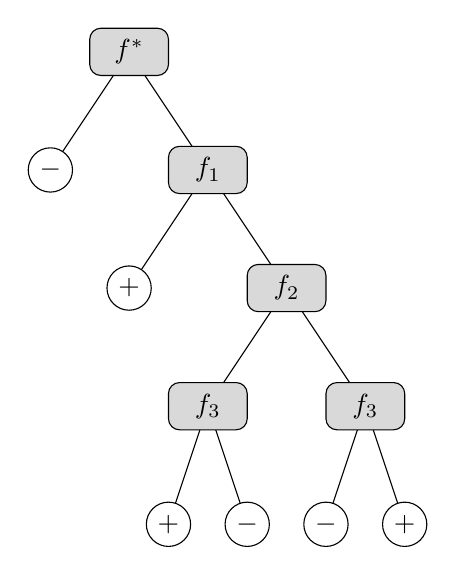
\begin{tikzpicture}[scale=1]
\draw (0,0.5)--(1,2)--(2,0.5)--(1,-1) (2,0.5)--(3,-1)--(4,-2.5)--(4.5,-4) (1.5,-4)--(2,-2.5)--(2.5,-4) (2,-2.5)--(3,-1) (3.5,-4)--(4,-2.5);
\draw[rounded corners,fill=gray!30!white] (0.5,1.7) rectangle (1.5,2.3) {};
\draw[rounded corners,fill=gray!30!white] (1.5,0.2) rectangle (2.5,0.8) {};
\draw[rounded corners,fill=gray!30!white] (2.5,-1.3) rectangle (3.5,-0.7) {};
\draw[rounded corners,fill=gray!30!white] (1.5,-2.8) rectangle (2.5,-2.2) {};
\draw[rounded corners,fill=gray!30!white] (3.5,-2.8) rectangle (4.5,-2.2) {};
\draw[fill=white] (0,0.5) circle (8pt) (1,-1) circle (8pt) (1.5,-4) circle (8pt) (2.5,-4) circle (8pt) (3.5,-4) circle (8pt) (4.5,-4) circle (8pt);
\node at (1,2) {$f^*$};
\node at (2,0.5) {$f_1$};
\node at (0,0.5) {$-$};
\node at (1,-1) {$+$};
\node at (3,-1) {$f_2$};
\node at (2,-2.5) {$f_3$};
\node at (4,-2.5) {$f_3$};
\node at (1.5,-4) {$+$};
\node at (2.5,-4) {$-$};
\node at (3.5,-4) {$-$};
\node at (4.5,-4) {$+$};
\end{tikzpicture}
\caption{The CI $E_3$ and the DT $T_3$.}\label{fig:E3T3}
\end{minipage}
\end{figure}

\begin{lemma}\label{lem:umss}
For every integer $k\geq 1$, the set of features $S_k$ is the only minimal support set in $S_k^*$ for $E_k$.
\end{lemma}

\begin{proof}
First we show that $S_k$ is a support set: let $e^-\in E^-_k$ and $e^+\in E^+_k$, by construction there is one feature $f\in S_k$ where $f(e^+)\neq f(e^-)$. 
Now it is time to show that, for any $i\in [k]$, the set $S_k^i=\{f_1,\ldots,\overline{f_i},\ldots,f_k,f^*\}=S_k^*\setminus \{f_i\}$ is not a support set for $E_k$. 
For $i\in [k-2]$, let $e^-_i$ and $e^+_i$ be the negative and the positive examples such that $f(e^-_i)=f(e^+_i)=1$ if $k$ is odd ($=0$ if $k$ is even) for every $f\in S_k^i$: 
$e^-_i$ and $e^+_i$ can not be distinguished by a feature in $S_k^i$ and so $S_k^i$ is not a support set (note there is one such pair $E_k$). 
For $i\in \{k-1,k\}$, let $e^-_i$ and $e^+_i$ be the negative and the positive examples in $D_k$ such that $f(e^-_i)=f(e^+_i)$ for every $f\in S_k^i$: $e^-_i$ and $e^+_i$ can not be distinguished by a feature in $S_k^i$ and so $S_k^i$ is not a support set (note there are two of such pairs in $E_k$).
\end{proof}

\begin{lemma}\label{lem:omss}
For every integer $k\geq 1$, a reduced DT $T$ with features in $S_k$ is a DT for $E_k$ if and only if $T$ is a complete DT of height $k+1$. In particular such DT has $2^{k+2}-1$ nodes ($2^{k+1}-1$ of those are inner nodes).
\end{lemma}

\begin{proof}
In this proof we assume that a leaf is either positive or negative depending on the parity of the number of right arcs present in the unique path from the root to that leaf. We start with the forward direction: let $T$ be a reduced DT that is not a complete DT of height $k+1$. Let $P$ be a path of $T$ from the root to a leaf $\ell$ of length at most $k$: at most $k-1$ features appear in $P$ and so there exists a feature $f_i\in S_k$ that does not appear in $P$. Since by Lemma~\ref{lem:umss} $S_k^i$ is not a support set for $E_k$, there exit a negative example $e^-$ and a positive example $e^+$ that can not be distinguished by $S_k^i$, this means that $\{e^-,e^+\}\subseteq E_T(\ell)$ and so $T$ is not a DT for $E_k$. 

In order to prove the backward direction, we assume that $T$ is a reduced and complete DT of height $k+1$ with features in $S_k$. Let $P$ be a path of $T$ from the root to a leaf $\ell$ of length $k+1$. Since $T$ is reduced, every feature of $S_k$ appears exactly once in $P$. Since by Lemma~\ref{lem:umss} $S_k$ is a support set, there is only one example $e_\ell$ that ends $\ell$, that is $e_\ell\in E_T(\ell)$. From this proof, it follows that every reduced DT $T$ with features in $\S_k$ for $E_k$ has $2^{k+2}-1$ nodes ($2^{k+1}-1$ of those are inner nodes).
\end{proof}

%GP: Let $\sigma$ be any bijection of the set $[k-2]$ and $\tau$ be any of the two bijections of the set $\{k-1,k\}$ and (arbitrarily) define $\sigma(k-1)=\tau(k-1)$. Let us describe a DT $T_{\sigma,\tau}$ as follows. The root of $r$ has feature $f^*$. The left child of $r$ is a negative leaf and the right child $v_1$ has feature $f_{\sigma(1)}$. For every $i\in [k-2]$, the left child of $v_i$ is a positive leaf and the right child $v_{i+1}$ has feature $f_{\sigma(i+1)}$. Finally $v_k$ and $v'_k$ are respectively the left and right child of $v_{k-1}$, both having feature $f_{\tau(k)}$. The children of $v_k$ and $v'_k$ are leaves that are either positive or negative depending on the parity of the number of right arcs present in the unique path from the root to that leaf. In particular note that $T_{\sigma,\tau}$ has $2k+5$ nodes ($k+2$ of those are inner nodes).

\note{A more general description of $T_k$ can be found commented.}

For every integer $k\geq 1$, let us describe a DT $T_k$ as follows. The root $r$ of $T_k$ has feature $f^*$. The left child of $r$ is a negative leaf and the right child $v_1$ has feature $f_1$. For every $i\in [k-2]$, the left child of $v_i$ is a positive leaf and the right child $v_{i+1}$ has feature $f_{i+1}$. Finally $v_k$ and $v'_k$ are respectively the left and right child of $v_{k-1}$, both having feature $f_k$. The children of $v_k$ and $v'_k$ are leaves that are either positive or negative depending on the parity of the number of right arcs present in the unique path from the root to that leaf. In particular note that $T_k$ has $2k+5$ nodes ($k+2$ of those are inner nodes). See Figure~\ref{fig:E3T3} for a visual representation of $T_3$.

\begin{lemma}\label{lem:emss}
For every integer $k\geq 1$, $T_k$ is a DT for $E_k$.
\end{lemma}

\begin{proof}
By construction, $r$ and its feature $f^*$ send every negative example to its left child $c_\ell$, which is a negative leaf, except for the two negative examples in $D_k$, that is, if $\{e_1^-,e_2^-\}=E^-_k\cap D_k$ then $E_{T_k}(c_\ell)=E^-_k\setminus \{e_1^-,e_2^-\}$ and $E_{T_k}(v_1)=E^+_k\cup \{e_1^-,e_2^-\}$.

Let $e$ be an example in $D_k$; by construction, for every $i\in [k-2]$ if $e\in  E_{T_k}(v_i)$ then $e\in E_{T_k}(v_{i+1})$ and by induction we obtain that $e\in E_{T_k}(v_{k-1})$. Let $e$ be an example in $\overline{D_k}$ and $j\in [k-2]$ be the minimum integer such that $f_j(e)=0$. This means that $e\not\in E_{T_k}(v_{j+1})$ and $e$ is classified by the left child of the node $v_j$. We have just proved that $D_k=E_{T_K}(v_{k-1})$ and that $T_k$ classifies $\overline{D_k}$. Now it is straightforward to show that the subtree of $T_k$ rooted at $v_{k-1}$ classifies $D_k$.
\end{proof}

Let $E$ be a CI and $S$ be a support set for $E$. We denote with $dts(E,S)$ the minimum size of a DT for $E$ that uses exactly all the features in $S$.
By Lemma~\ref{lem:omss}, we have that $dts(E_k,S_k)=2^{k+2}-1$. Moreover, since by Lemma~\ref{lem:emss} $T_k$ is a DT for $E_k$, we have that $dts(E_k,S^*_k)\leq |T_k|=2k+5$.
In conclusion we have that $$\frac{dts(E_k,S_k)}{dts(E_k,S^*_k)}\geq \frac{2^{k+2}+1}{2k+5}\approx \frac{2^{k+1}}{k}.$$

\subsection{For Height}

For every integer $k\geq 1$, let us describe a DT $T^k$ as follows. The tree $T^k$ has $v_1$ as root. For every $i\in [k]$, the node $v_i$ has $v_{2i}$ and $v_{2i+1}$ as left child and right child respectively. Moreover, if $i\leq k$, the node $v_i$ has feature $f_i$ and is a leaf otherwise (negative if $i$ is even and positive if $i$ is odd). Note that $T^k$ has height $log(k)+1$.

Let $F_k$ be the set of all the examples in $E_k$ that are classified by $T^k$ and denote by $\overline{F_k}=E_k\setminus F_k$. Now we are ready to define a new feature $f'$ follows: $f'(e)=0$ if $e\in F_k$ and $f'(e)=1$ otherwise. We also introduce another new feature $f''$ as follows: $f''(e)=0$ if either $e\in F_k$ or $e$ is a negative example and $f''(e)=1$ otherwise.
For simplicity the set $S'_k$ denotes $\{f_1,\ldots,f_k,f',f''\}$.

For every integer $k\geq 1$, let us describe a DT $T^k_*$ as follows. The root of $r$ has feature $f'$ and its left branch is the DT $T^k$. The right child of $r$ is a node $u$ with feature $f''$. The left/right child of $u$ is a negative/positive leaf. In particular note that $T^k_*$ has height $log(k)+2$. See Figure~\ref{fig:E3T3*} for a visual representation of $E_3$, its decomposition in $F_3$ and $\overline{F_3}$ and the DTs $T^3$ and $T^3_*$.

\begin{figure}[h]
\small
\begin{minipage}{0.3\linewidth}
\centering
\begin{tabular}{ccc|c|c|cc}
$f_1$ & $f_2$ & $f_3$ & $f'$ & $f''$ &\\
\hline
$0$ & $0$ & $1$ & $0$ & $0$ & $-$ \\
$0$ & $1$ & $1$ & $0$ & $0$ & $+$ & {$F_3$}\\
$1$ & $0$ & $0$ & $0$ & $0$ & $-$ \\
$1$ & $0$ & $1$ & $0$ & $0$ & $+$ \\
\hline
$0$ & $0$ & $0$ & $1$ & $1$ & $+$ \\
$0$ & $1$ & $0$ & $1$ & $0$ & $-$ \\
$1$ & $1$ & $0$ & $1$ & $1$ & $+$ & $\overline{F_3}$\\
$1$ & $1$ & $1$ & $1$ & $0$ & $-$
\end{tabular}
\end{minipage}%
\begin{minipage}{0.5\linewidth}
\centering
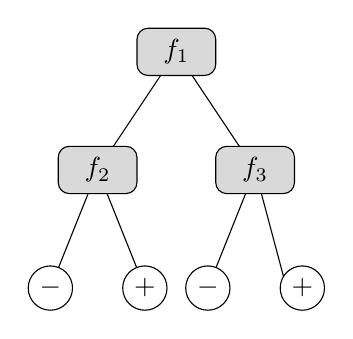
\begin{tikzpicture}[scale=1]
\draw (-0.6,-1)--(0,0.5)--(1,2)--(2,0.5)--(2.4,-1) (0,0.5)--(0.6,-1) (2,0.5)--(1.4,-1);
\draw[rounded corners,fill=gray!30!white] (0.5,1.7) rectangle (1.5,2.3) {};
\draw[rounded corners,fill=gray!30!white] (-0.5,0.2) rectangle (0.5,0.8) {};
\draw[rounded corners,fill=gray!30!white] (1.5,0.2) rectangle (2.5,0.8) {};
\draw[fill=white] (1.4,-1) circle (8pt);
\draw[fill=white] (2.6,-1) circle (8pt);
\draw[fill=white] (-0.6,-1) circle (8pt);
\draw[fill=white] (0.6,-1) circle (8pt);
\node at (1,2) {$f_1$};
\node at (0,0.5) {$f_2$};
\node at (2,0.5) {$f_3$};
\node at (1.4,-1) {$-$};
\node at (2.6,-1) {$+$};
\node at (-0.6,-1) {$-$};
\node at (0.6,-1) {$+$};
\end{tikzpicture}
\end{minipage}%
\begin{minipage}{0.1\linewidth}
\centering
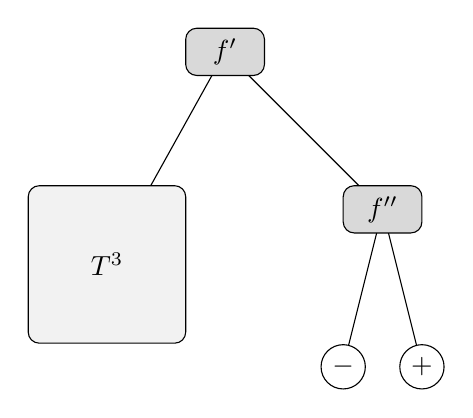
\begin{tikzpicture}[scale=1]
\draw (-1.5,-0.7)--(0,2)--(2,0)--(1.5,-2) (2,0)--(2.5,-2);
\draw[rounded corners,fill=gray!30!white] (-0.5,1.7) rectangle (0.5,2.3) {};
\draw[rounded corners,fill=gray!30!white] (1.5,-0.3) rectangle (2.5,0.3) {};
\draw[rounded corners,fill=gray!10!white] (-2.5,-1.7) rectangle (-0.5,0.3) {};
\draw[fill=white] (1.5,-2) circle (8pt);
\draw[fill=white] (2.5,-2) circle (8pt);
\node at (0,2) {$f'$};
\node at (2,0) {$f''$};
\node at (-1.5,-0.7) {$T^3$};
\node at (1.5,-2) {$-$};
\node at (2.5,-2) {$+$};
\end{tikzpicture}
\end{minipage}
\caption{The CI $E_3$, the DT $T^3$ and the DT $T^3_*$} \label{fig:E3T3*}
\end{figure}

\begin{lemma}\label{lem:humss}
For every integer $k\geq 1$, the set of features $S_k$ is the only minimal support set in $S'_k$ for $E_k$.
\end{lemma}

\begin{proof}
By Lemma~\ref{lem:umss}, the set $S_k$ is a support set.
Now it is time to show that, for every $i\in [k]$, the set $S^i_k=\{f_1,\ldots,\overline{f_i},\ldots,f_k,f',f''\}=S'_k\setminus \{f_i\}$ is not a support set for $E_k$. 

Let $e_i$ be an example of $F_k$ be such that, in $T^k$, $e_i$ ends in a leaf $\ell_i$ which has $v_i$ as an ancestor. Let $P_i$ be the path from $\ell_i$ to $v_i$.
Since $T^k$ has height $log(k)<k$ there is at least a feature in $S_k$ that does not appear in the path from $r$ to $\ell_i$: therefore such example $e_i$ always exists.

Let $Q_i$ be the path from the child of $v_i$ that is not an ancestor of $\ell_i$ to a leaf $\ell'_i$ such that for every left arc $uw$ of $Q_i$ then $feat(u)(e_i)=0$ and for every right arc $uw$ of $Q_i$ then $feat(u)(e_i)=1$.
Let $e'_i$ be the example in $E_k$ such that $f_j(e'_i)=f_j(e_i)$ for every $j\in [k]\setminus \{i\}$ and $f_i(e'_i)=1-f_i(e_i)$. Now it is crucial to note that $e'_i\in F_k$: indeed $e'_i$ ends in the $\ell'_i$ (and its sign is different from the one of $\ell_i$).
Since $e_i$ and $e'_i$ are both examples of $F_k$, by construction $e_i$ and $e'_i$ can not be distinguished by either $f'$ or $f''$.

This means that $e_i$ and $e'_i$ can not be distinguished by a feature in $S^i_k$ and so $S^i_k$ is not a support set.
\end{proof}

\begin{lemma}\label{lem:hemss}
For every integer $k\geq 1$, $T^k_*$ is a DT for $E_k$.
\end{lemma}

\begin{proof}
By construction, $r$ and its feature $f'$ send every example of $F_k$ to its left child and every other example, that is $\overline{F_k}$, to the right child. By definition, the set $F_k$ is classified by $T^k$ and, by construction, the subtree of $T^k_*$ rooted at the right child $u$ of $r$ classifies $\overline{F_k}$.
Therefore, $T^k_*$ classifies $F_k\cup \overline{F_k}=E_k$.
\end{proof}

Let $E$ be a CI and $S$ be a support set for $E$. We denote with $dth(E,S)$ the minimum height of a DT for $E$ that uses exactly all the features in $S$.
By Lemma~\ref{lem:omss}, we have that $dth(E_k,S_k)=k+1$. Moreover, since by Lemma~\ref{lem:hemss} $T^k_*$ is a DT for $E_k$, we have that $dth(E_k,S'_k)\leq |T^k_*|=log(k)+2$.
In conclusion we have that $$\frac{dth(E_k,S_k)}{dth(E_k,S'_k)}\geq \frac{k+1}{log(k)+2}\approx \frac{k}{log(k)}.$$






%\bibliography{literature}
\end{document}